\section{Introduzione}
\begin{frame}{}

  \textsc{Green Together} permette di semplificare la trasmissione dell'informazione da e verso i cittadini, includendoli e ascoltandoli.
  \pause
  \bigskip

  Un canale a doppio flusso che semplifica e centralizza la comunicazione.
  \pause

\end{frame}
\begin{frame}
  Non sarà più necessario analizzare flussi di mail per capire quali siano le richieste più ricorrenti e cosa stia davvero a cuore ai cittadini
  \pause

  Con un' unica piattaforma sarà possibile esercitare:
  \textbf{informazione},  \textbf{trasparenza} e  \textbf{partecipazione}
\end{frame}
\begin{frame}{Attori}
  Gli attori che entrano in gioco sono:
  \begin{description}
    \item[I cittadini] che usufruiscono dei servizi ambientali di zona
    \item[L'azienda] che gestisce questi servizi
  \end{description}


\end{frame}

\begin{frame}{Struttura}

  \begin{figure}

    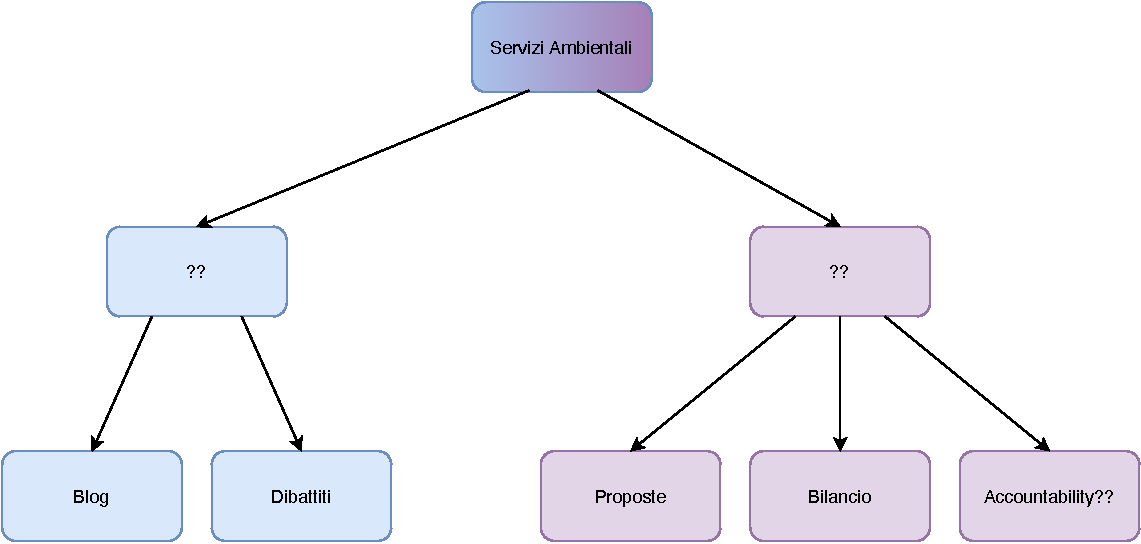
\includegraphics[width=\textwidth]{Diagramma}
  \end{figure}

\end{frame}
\begin{frame}{Funzioni}
  \textbf{Comunichiamo}
  \begin{description}
    \item[Blog] Consente all'azienda di comunicare con i cittadini
    \item[Dibattiti] Consente ai cittadini di comunicare reciprocamente e con l'azienda
  \end{description}
  \textbf{Decidiamo}

  \begin{description}
    \item[Proposte] Consente ai cittadini e all'azienda di fare proposte e votarle
    \item[Bilancio] Una volta selezionate alcune proposte consente di ripartire un budget sui vari progetti
    \item[Accountability] Monitora lo stato dei progetti sovvenzionati
  \end{description}
\end{frame}